\begin{center}
	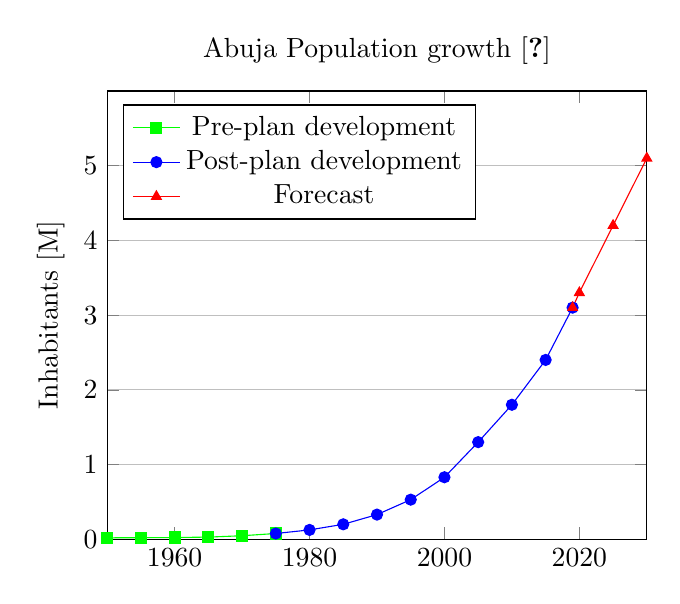
\begin{tikzpicture}[>=latex]
		\begin{axis}[
				title={Abuja Population growth \cite{WorldPopulationReview:Abuja}},
				style={/pgf/number format/1000 sep=},
				ylabel={Inhabitants [M]},
				xmin=1950, xmax=2030,
				ymin=0, ymax=6,
				xtick={1960,1980,2000,2020},
				ytick={0,1,2,3,4,5},
				legend pos=north west,
				ymajorgrids=true
			]
			\addplot[color=green,mark=square*] coordinates {
					(1950,0.019)(1955,0.021)(1960,0.023)(1965,0.029)(1970,0.047)(1975,0.077)
				};
			\addplot[color=blue,mark=otimes*] coordinates {
					(1975,0.077)(1980,0.125)(1985,0.2)(1990,0.33)(1995,0.53)(2000,0.83)(2005,1.3)(2010,1.8)(2015,2.4)(2019,3.1)
				};
			\addplot[color=red,mark=triangle*] coordinates {
					(2019,3.1)(2020,3.3)(2025,4.2)(2030,5.1)
				};
			\legend{Pre-plan development,Post-plan development,Forecast}				
		\end{axis}
	\end{tikzpicture}	
\end{center}
